%===============================================================================
%===============================================================================
%
\clearpage
%
\subsection{Example-0005 \texttt{[VALIDATED]}}
%
Example uses two user-defined (2d and 3d) unregular meshes and solves a patch test  in form of a static problem, i.e., applies
the boundary conditions in one step.
Here, a Laplace problem with two Dirichlet boundary conditions is solved.
The analytical solution for this setting is known and results in a linear distribution of the scalar Laplace parameter $u$.
The numerical solution has to recover this the linear distribution in order to pass the Patch test.
2d and 3d meshes are according to MacNeil and Harder (1985).
%
%===============================================================================
%
\subsubsection{Mathematical model - 2D}
%
We solve the following scalar equation,
%
\begin{align}
    \nabla \cdot \nabla u = 0 & &&\Omega = [0, 0.24] \times [0, 0.12],
\end{align}
%
with boundary conditions
%
\begin{align}
    u = 0      & &&x = 0, \\
    u = 1      & &&x = 0.24.
\end{align}
%
No material parameters to specify.
%
%===============================================================================
%
\subsubsection{Mathematical model - 3D}
%
We solve the following scalar equation,
%
\begin{align}
    \nabla \cdot \nabla u = 0 & &&\Omega = [0, 1] \times [0, 1] \times [0, 1],
\end{align}
%
with boundary conditions
%
\begin{align}
    u = 0      & &&x = 0, \\
    u = 1      & &&x = 1.
\end{align}
%
No material parameters to specify.
%
%===============================================================================
%
\subsubsection{Computational model}
%
\begin{itemize}
    \item{Commandline arguments are:}
        \subitem{integer: dimension (2: 2d; 3: 3d)}
        \subitem{integer: interpolation order (1: linear; 2: quadratic)}
        \subitem{integer: solver type (0: direct; 1: iterative)}
    \item{Commandline arguments for tests are:}
        \subitem{2 1 0}
        \subitem{2 2 0}
        \subitem{2 1 1}
        \subitem{2 2 1}
        \subitem{3 1 0}
        \subitem{3 2 0}
        \subitem{3 1 1}
        \subitem{3 2 1}
\end{itemize}
%
%===============================================================================
%
\subsubsection{Result summary}
%
Since the analytical result is known and the numerical results have to recover the linear distribution of $u$, the comparisons are done with the analytical solution.
%
\verbatiminput{examples/example-0005/results/results.summary}
\verbatiminput{examples/example-0005/results/failed.tests}
%
\begin{figure}[h!]
    \centering 
    \includegraphics[width=0.9\columnwidth]{examples/example-0005/doc/figures/2d_mesh.eps} 
    \caption{2D geometry and mesh.}
    \label{3d-mesh-fig}
\end{figure}
%
\begin{figure}[h!]
    \centering 
    \includegraphics[width=0.9\columnwidth]{examples/example-0005/doc/figures/iron_reference_2D.eps} 
    \caption{2D results, iron reference w/ command line arguments [2 2 0].}
    \label{example-0005-iron-2D-reference-fig}
\end{figure}
%
\begin{figure}[h!]
    \centering 
    \includegraphics[width=0.9\columnwidth]{examples/example-0005/doc/figures/current_run_d2_i2_s0.eps} 
    \caption{2D results, current run w/ command line arguments [2 2 0].}
    \label{example-0005-current-run-2D-fig}
\end{figure}
%
\begin{figure}[h!]
    \centering 
    \includegraphics[width=0.9\columnwidth]{examples/example-0005/doc/figures/3d_mesh.eps} 
    \caption{3D geometry (unit cube) and mesh.}
    \label{3d-mesh-fig}
\end{figure}
%
\begin{figure}[h!]
    \centering 
    \includegraphics[width=0.9\columnwidth]{examples/example-0005/doc/figures/iron_reference_3D.eps} 
    \caption{3D results, iron reference w/ command line arguments [3 2 0].}
    \label{example-0005-iron-3D-reference-fig}
\end{figure}
%
\begin{figure}[h!]
    \centering 
    \includegraphics[width=0.9\columnwidth]{examples/example-0005/doc/figures/current_run_d3_i2_s0.eps} 
    \caption{3D results, current run w/ command line arguments [3 2 0].}
    \label{example-0005-current-run-3D-fig}
\end{figure}
%
%===============================================================================
%===============================================================================
